\documentclass[aspectratio=1611, 9pt]{beamer}

\usepackage[utf8]{inputenc} % Only once, at the top
\usepackage{lmodern,textcomp}

\usepackage{subfig}
\usepackage{amssymb,amsmath,mathtools}
\usepackage{amsfonts,booktabs}
\usepackage{lmodern,textcomp}
\usepackage{color}
\usepackage{tikz}
\usepackage{natbib}
\usepackage{multicol}
\usepackage{graphicx}
\usepackage{caption}
\usepackage{hyperref}         % Make links clickable
\usepackage{url}
\usepackage{amsmath, amssymb, amsfonts}
\usepackage{lmodern}

\usetheme{Madrid}
\usecolortheme{default}

\title[SES4U]{History of Space Science to 1700s}
\subtitle{Myths + Geocentric System + Heliocentric System}
\author{Qinghao Hu}

\begin{document}

\frame{\titlepage}

\section{Expectation}
\begin{frame}
  \frametitle{Expectations}
  \begin{enumerate}
    \item Describe how early cultures created \textcolor{red}{myths} to explain the universe.
    \item Explain the differences between the \textcolor{red}{Geocentric System} and \textcolor{red}{Heliocentric System}.
    \item Describe how humans' understanding of the universe developed in \textcolor{red}{chronological order}.
    \item Describe how each scientist contributed to the \textcolor{red}{Geocentric} and \textcolor{red}{Heliocentric} systems.
  \end{enumerate}
\end{frame}

\section{Chapter I}
\begin{frame}
  \frametitle{The Start of Space Science: Myths}
  \begin{center}
    \textbf{The origin of space science lies in myths and storytelling.}
  \end{center}
\end{frame}

\section{Introduction}
\begin{frame}
  \frametitle{Myth}
  \begin{columns}
    \column{0.50\textwidth}
    \begin{center}
      At the beginning of mankind, early civilizations did not understand modern science. 
      They created \textcolor{red}{stories and myths} to explain the universe.
      
      \begin{exampleblock}{Examples}
        Two examples are taken from Grade 10 English.
      \end{exampleblock}
    \end{center}

    \column{0.40\textwidth}
    \begin{center}
      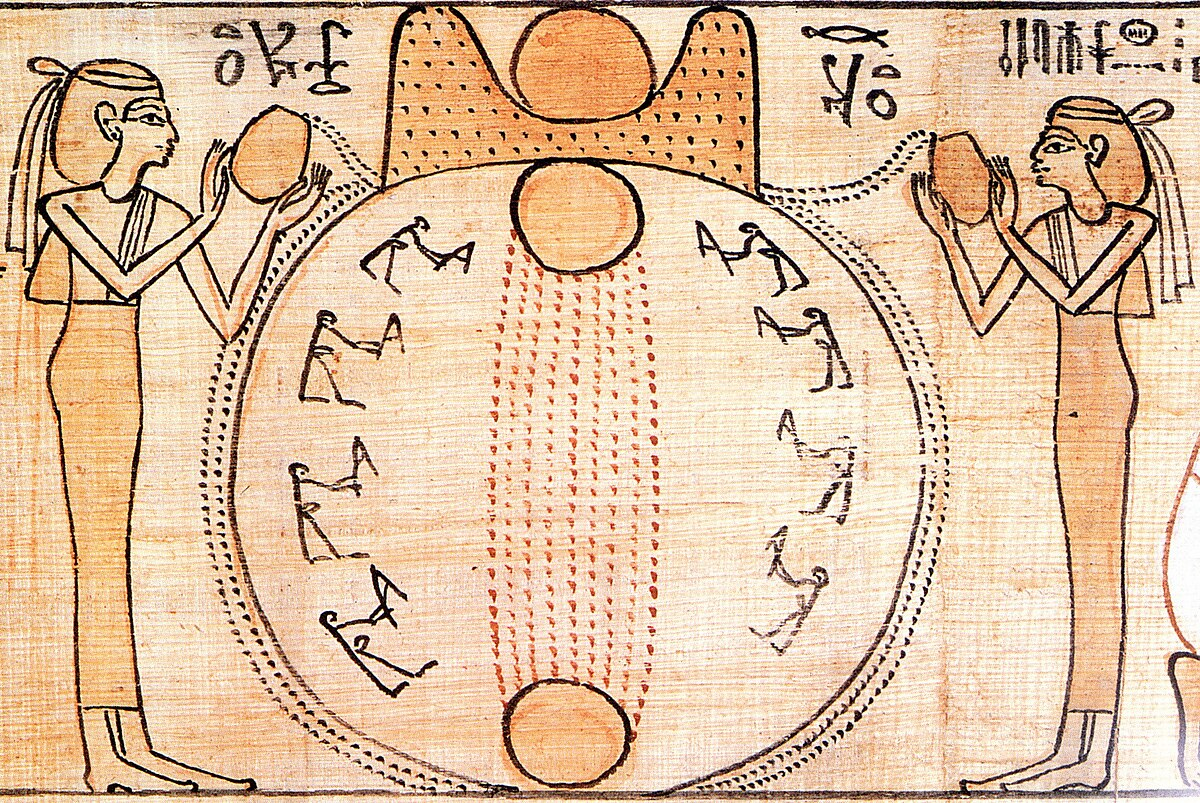
\includegraphics[width=0.9\textwidth]{pictures/myth1.jpg}
      \captionof{figure}{Ancient Egyptian Creation Myth}
    \end{center}
  \end{columns}
\end{frame}

\section{Myth Examples}
\begin{frame}
  \frametitle{Example I: Pangu Creates the World}
  \begin{columns}
    \column{0.55\textwidth}
    \begin{itemize}
      \item From \textcolor{red}{Chinese culture}.
      \item Pangu used his hands and legs to break the chaos.
      \item His \textcolor{red}{left eye} became the \textbf{Sun}.
      \item His \textcolor{red}{right eye} became the \textbf{Moon}.
      \item His \textcolor{red}{flesh} became the \textbf{soil}.
    \end{itemize}

    \column{0.40\textwidth}
    \begin{center}
      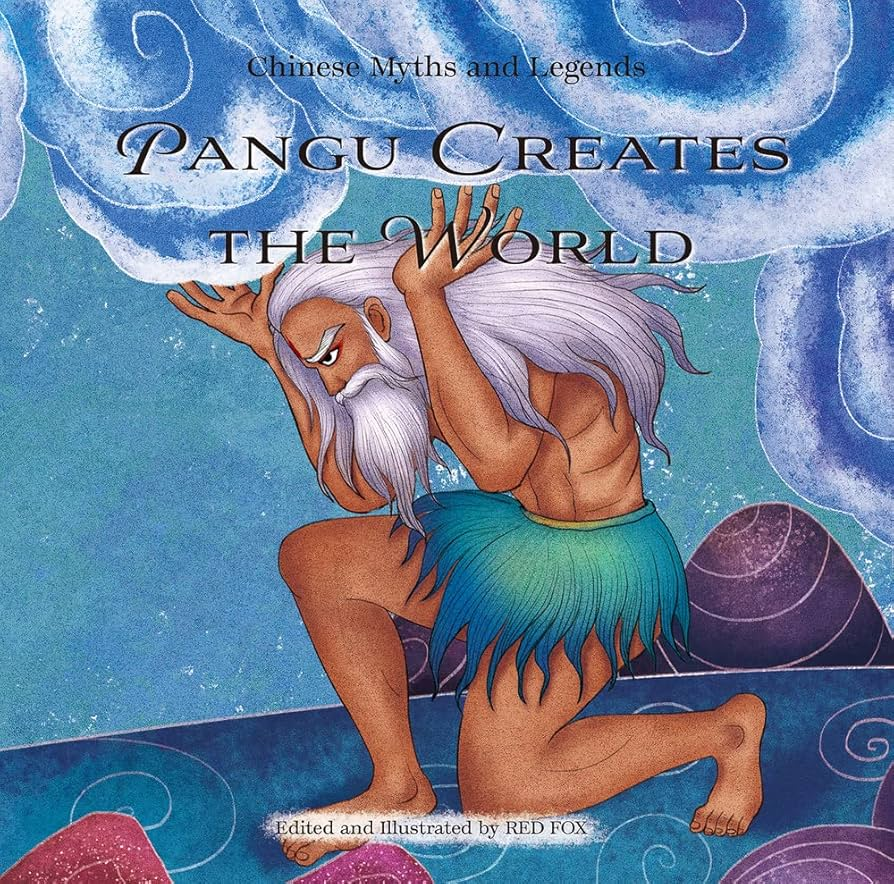
\includegraphics[width=1.0\textwidth]{pictures/myth2.jpg}
      \captionof{figure}{Pangu creates the Earth (from \textit{Amazon})}
    \end{center}
  \end{columns}
\end{frame}

\begin{frame}
  \frametitle{Example II: The Turtle Island Myth}
  \begin{columns}
    \column{0.50\textwidth}
    \begin{itemize}
     \item From \textcolor{red}{Indigenous peoples of North America}.
    \item The Earth was formed on the back of a giant \textcolor{red}{turtle} -- "Turtle Island".
    \item A woman gave birth to \textbf{twins}.
    \item The \textcolor{red}{Good Twin} placed the \textbf{Sun} in the sky for \textcolor{red}{warmth and daylight}.
    \item The \textcolor{red}{Bad Twin} placed the \textbf{Moon} in the sky for \textcolor{red}{cold and darkness}.
    \item Such myths explained the \textcolor{red}{cosmos} before scientific astronomy.
    \end{itemize}

    \column{0.40\textwidth}
    \begin{center}
      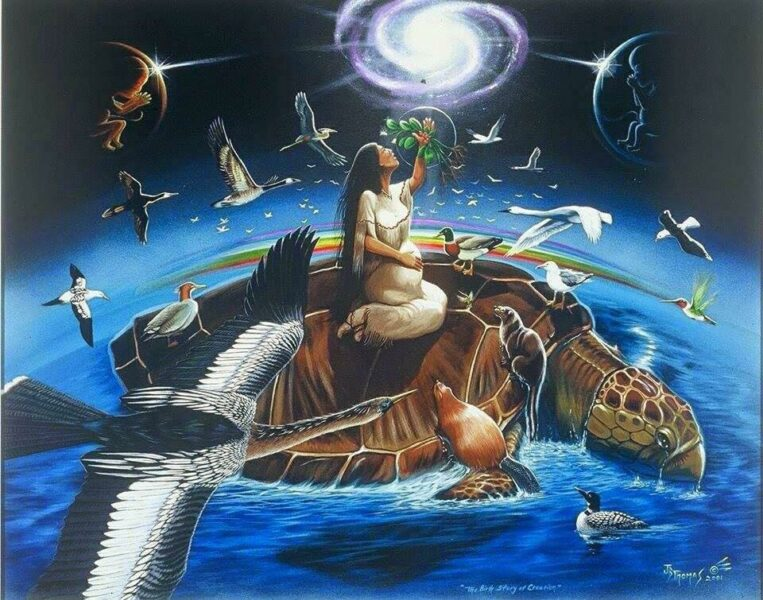
\includegraphics[width=1.0\textwidth]{pictures/myth3.jpg}
      \captionof{figure}{From \textit{Sequoia Proudly Indigenous}}
    \end{center}
  \end{columns}
\end{frame}

\section{Ancient Greek}
\begin{frame}
  \begin{center}
    \textbf{Ancient Greek Space Science and the Geocentric Model}
  \end{center}
\end{frame}

\begin{frame}
  \frametitle{Eudosus (390–337 BCE): Concentric Spheres Geocentric System}
  \begin{columns}
    \column{0.50\textwidth}
    \begin{itemize}
      \item Mathematician and astronomer.
      \item Proposed the first geometric model of planetary motion.
      \item Used \textcolor{red}{27 concentric spheres} with Earth at the center.
      \item The first people to use \textcolor{red}{mathematics and geometry} to analyze the heavens or Universe.
    \end{itemize}
    \begin{alertblock}{Note}
      Spheres were primarily \textcolor{red}{mathematical tools}, not physical objects.
    \end{alertblock}

    \column{0.40\textwidth}
    \begin{center}
      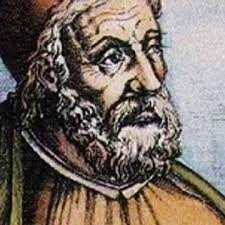
\includegraphics[width=0.9\textwidth]{pictures/eudosus.jpg}
      \captionof{figure}{Eudosus (from Locklin on Science)}
    \end{center}
  \end{columns}  
\end{frame}

\begin{frame}
  \begin{block}{Search: Please go to the first Link}
    You should go to the google classroom. There is a tab post by me!
  \end{block}

  \begin{center}
  \textbf{By the way, did you see this model in any movie?}
  \end{center}
\end{frame}

\begin{frame}
  \frametitle{Game of Throne}

  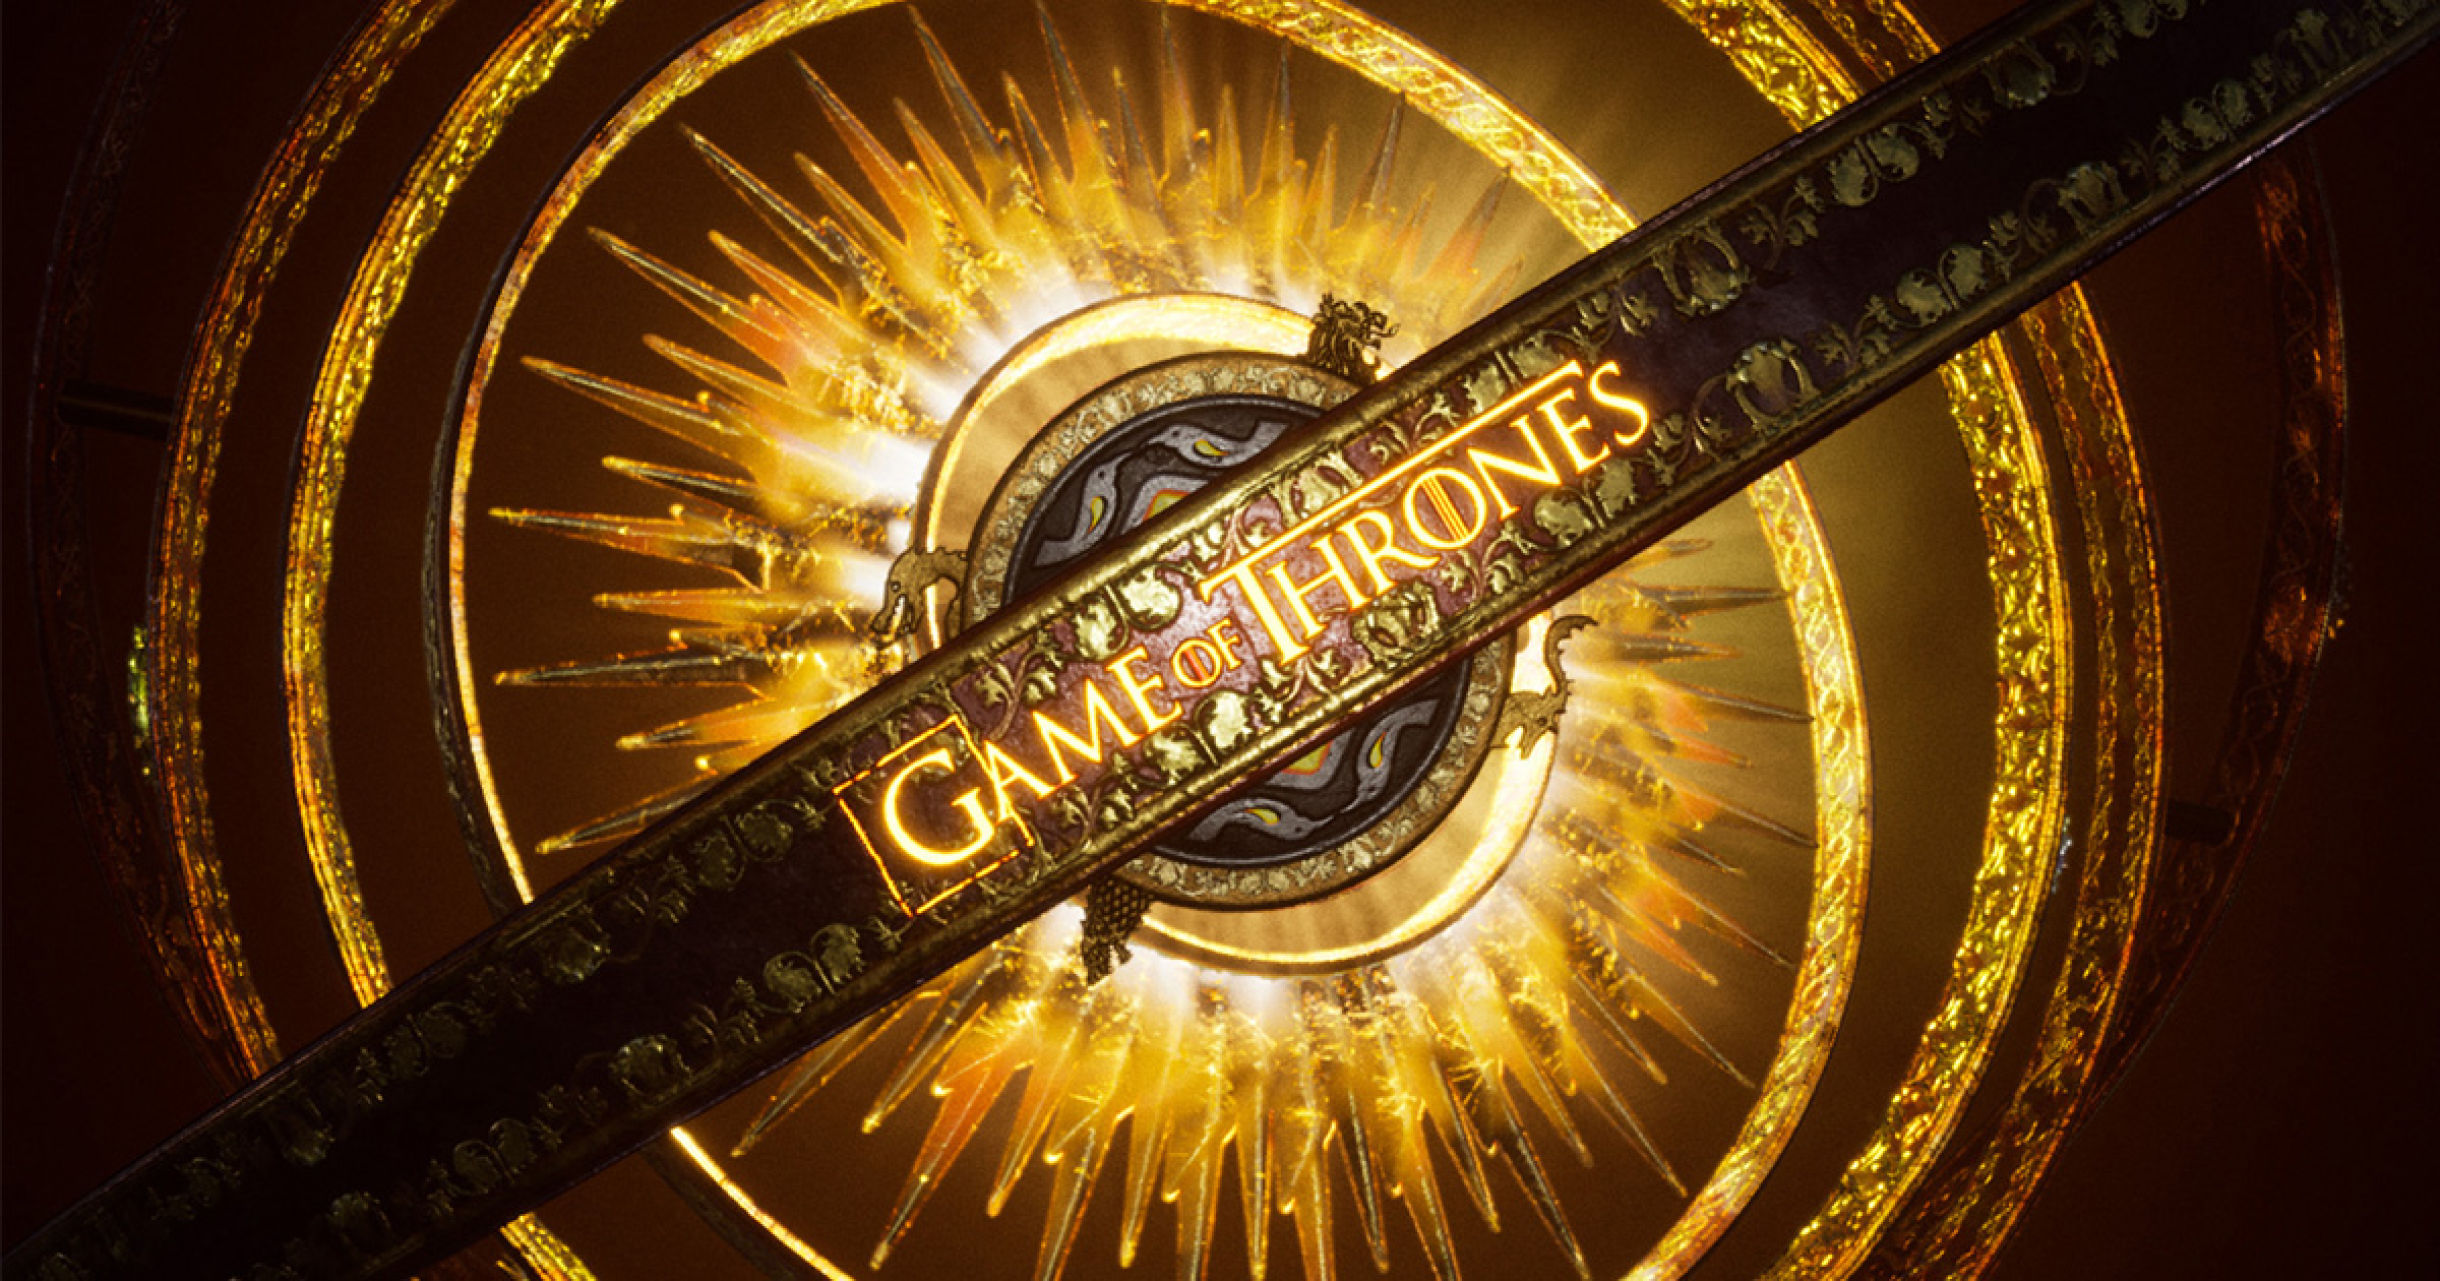
\includegraphics[width=\textwidth]{pictures/gameOfThrone.jpg}
  \captionof{figure}{The screenshot from the "Game of Thrones"}

\end{frame}

\begin{frame}
  \frametitle{Aristotle (384–322 BCE): The Second Geocentric System}
  \begin{columns}
    \column{0.45\textwidth}
    \begin{itemize}
      \item Known as \textbf{The Father of Western Philosophy}.
      \item Ancient Greek philosopher.
    \end{itemize}
    \begin{block}{Interesting Fact}
      He liked to bathe in olive oil and then sell it to others.
    \end{block}

    \column{0.40\textwidth}
    \begin{center}
      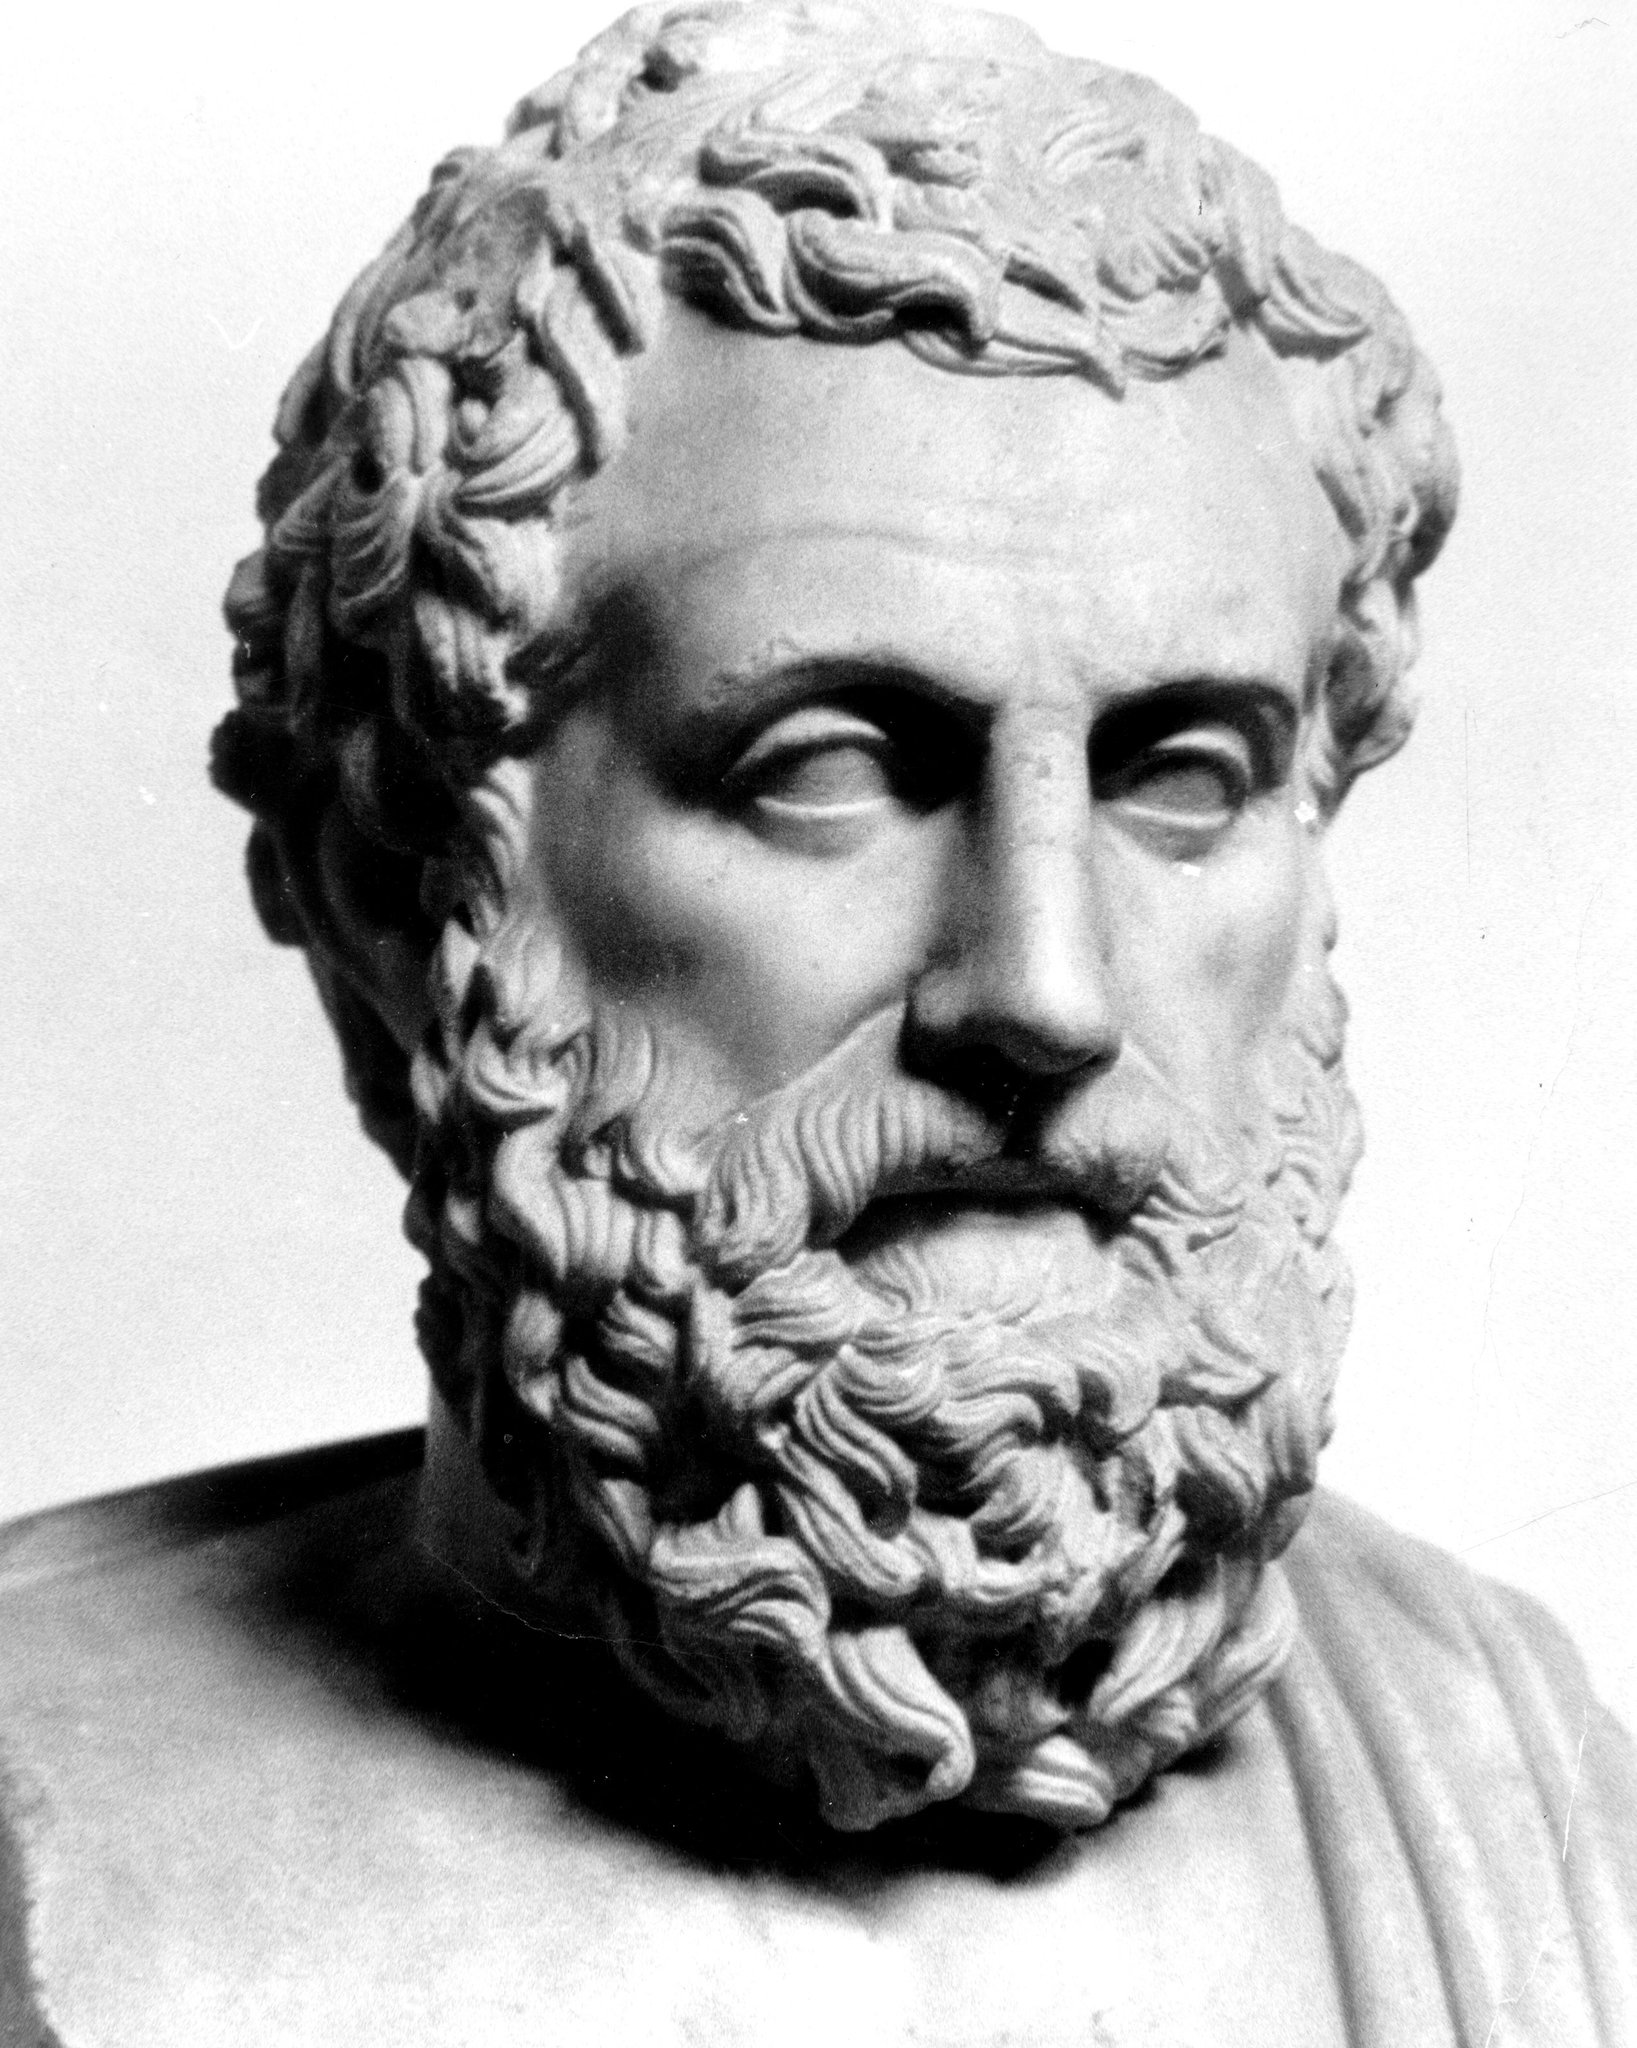
\includegraphics[width=0.9\textwidth]{pictures/aristotle.jpg}
      \captionof{figure}{Aristotle (from \textit{The New York Times})}
    \end{center}
  \end{columns}
\end{frame}

\begin{frame}
  \frametitle{"On the Heavens"}
  \begin{columns}
    \column{0.50\textwidth}
    \begin{itemize}
      \item \textcolor{red}{"On the Heavens"} is Aristotle's chief cosmological treatise.
      \item Expanded \textcolor{red}{Eudosus's model} using \textcolor{red}{~55 concentric spheres}.
      \item Earth is a \textcolor{red}{sphere} and \textcolor{red}{stationary} at the universe's center.
      \item Everything else travels in \textcolor{red}{perfect circular orbits}.
      \item Universe is \textcolor{red}{spherical and finite}.
    \end{itemize}

    \column{0.40\textwidth}
    \begin{center}
      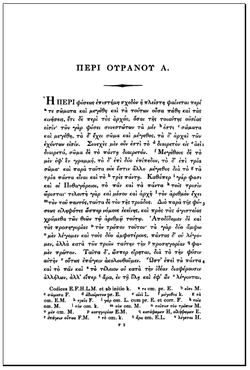
\includegraphics[width=0.80\textwidth]{pictures/heaven.png}
      \captionof{figure}{Page one of \textit{"On the Heavens"}}
    \end{center}
  \end{columns}
\end{frame}

\begin{frame}
  \frametitle{Ptolemy (100–170 AD): The Final Geocentric System}
  \begin{columns}
    \column{0.50\textwidth}
    \begin{itemize}
      \item Developed the \textcolor{red}{\textbf{Geocentric Model}}.
      \item Model dominated for over 1400 years.
      \item Mathematician, astronomer, geographer, and music theorist.
    \end{itemize}

    \column{0.45\textwidth}
    \begin{center}
      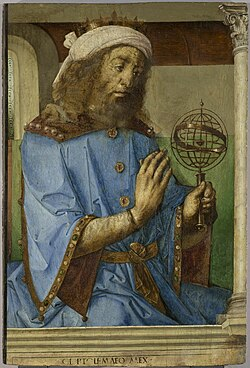
\includegraphics[width=0.8\textwidth]{pictures/Ptolemy.jpg}
      \captionof{figure}{Ptolemy (from University of Toronto)}
    \end{center}
  \end{columns}
\end{frame}

\begin{frame}
  \frametitle{Retrograde motion}
  \begin{center}
    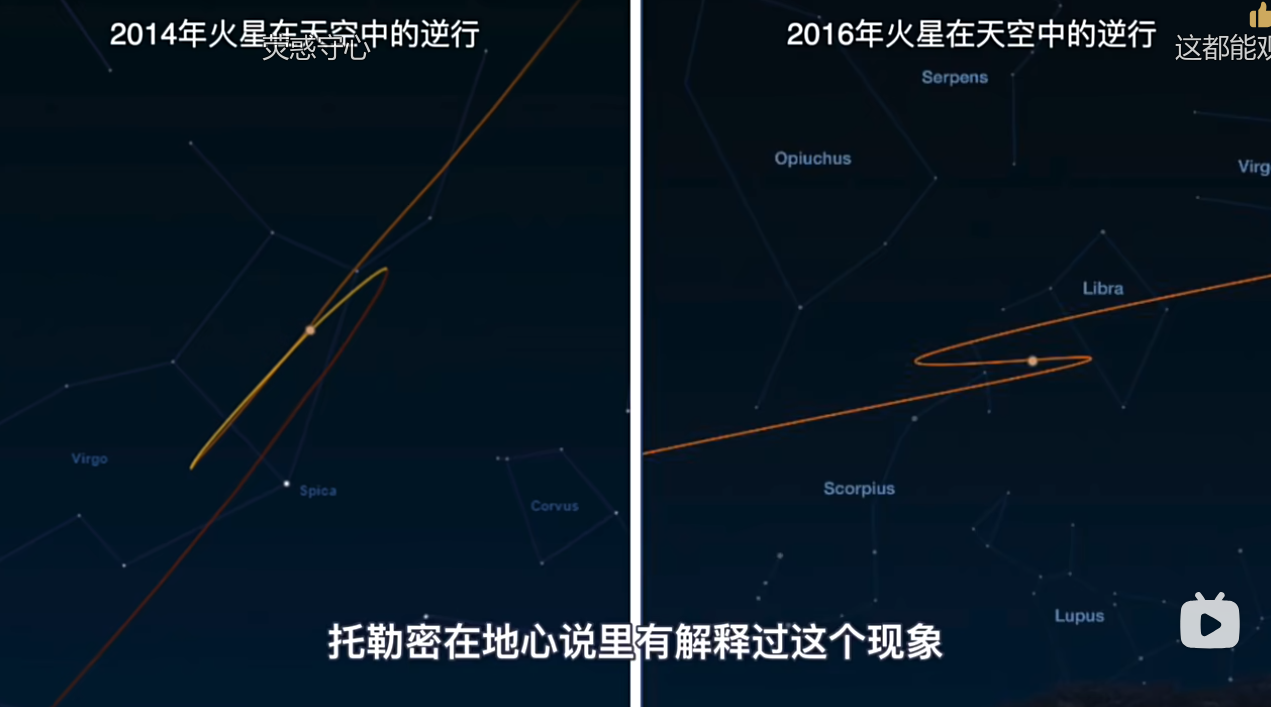
\includegraphics[width=\textwidth]{pictures/2025-09-27_21-33-05.png}
    \captionof{figure}{This is the Screenshot from Bilibili by me}
  \end{center}
\end{frame}

\begin{frame}
  \frametitle{Almagest}
  \begin{columns}
    \column{0.50\textwidth}
    \begin{itemize}
      \item Most famous work by Ptolemy.
      \item Introduced \textcolor{red}{epicycles} to explain \textcolor{red}{retrograde motion}.
      \item Model accurately predicted planetary positions.
      \item Planetary orbits were \textcolor{red}{circular}, not spherical.
    \end{itemize}
    \begin{alertblock}{Google}
      Go to the second link in my tab!
    \end{alertblock}

    \column{0.45\textwidth}
    \begin{center}
      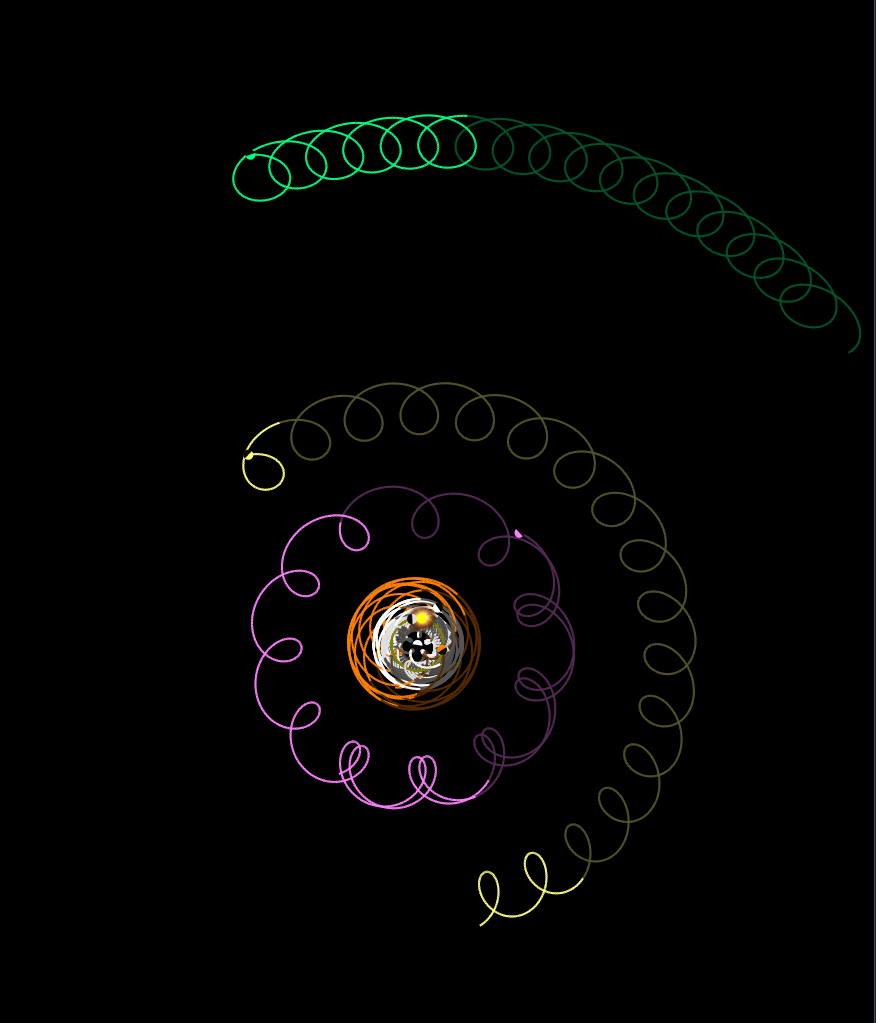
\includegraphics[width=0.9\textwidth]{pictures/geocentric.png}
      \captionof{figure}{Screenshot from orbitsimulator.com by author}
    \end{center}
  \end{columns}
\end{frame}

\begin{frame}
  \frametitle{Student Activity I}
  \begin{center}
   \textbf{According to the animation, try to summary the characteristics of "Geocentric System"}\\
    \textbf{Is this model easy to use?}\\
    \textbf{Is this model easy to understand?}\\
  \end{center}
\end{frame}

\section{Heliocentric System}
\begin{frame}
  \frametitle{Introduction to Heliocentric System}
  \begin{center}
    \textbf{The Sun-centered Universe}
  \end{center}
\end{frame}

\begin{frame}
  \frametitle{Copernicus and the Sun-Centered Universe}
  \begin{columns}
    \column{0.50\textwidth}
    \begin{itemize}
      \item Nicolaus Copernicus
      \item Born into a wealthy family
      \item Doctorate in \textcolor{red}{Canon Law}
      \item He read a lot of cosmic books from Ptolemy
    \end{itemize}
    \begin{block}{Interesting Fact}
      He was a \textcolor{red}{clergyman}.
    \end{block}

    \column{0.40\textwidth}
    \begin{center}
      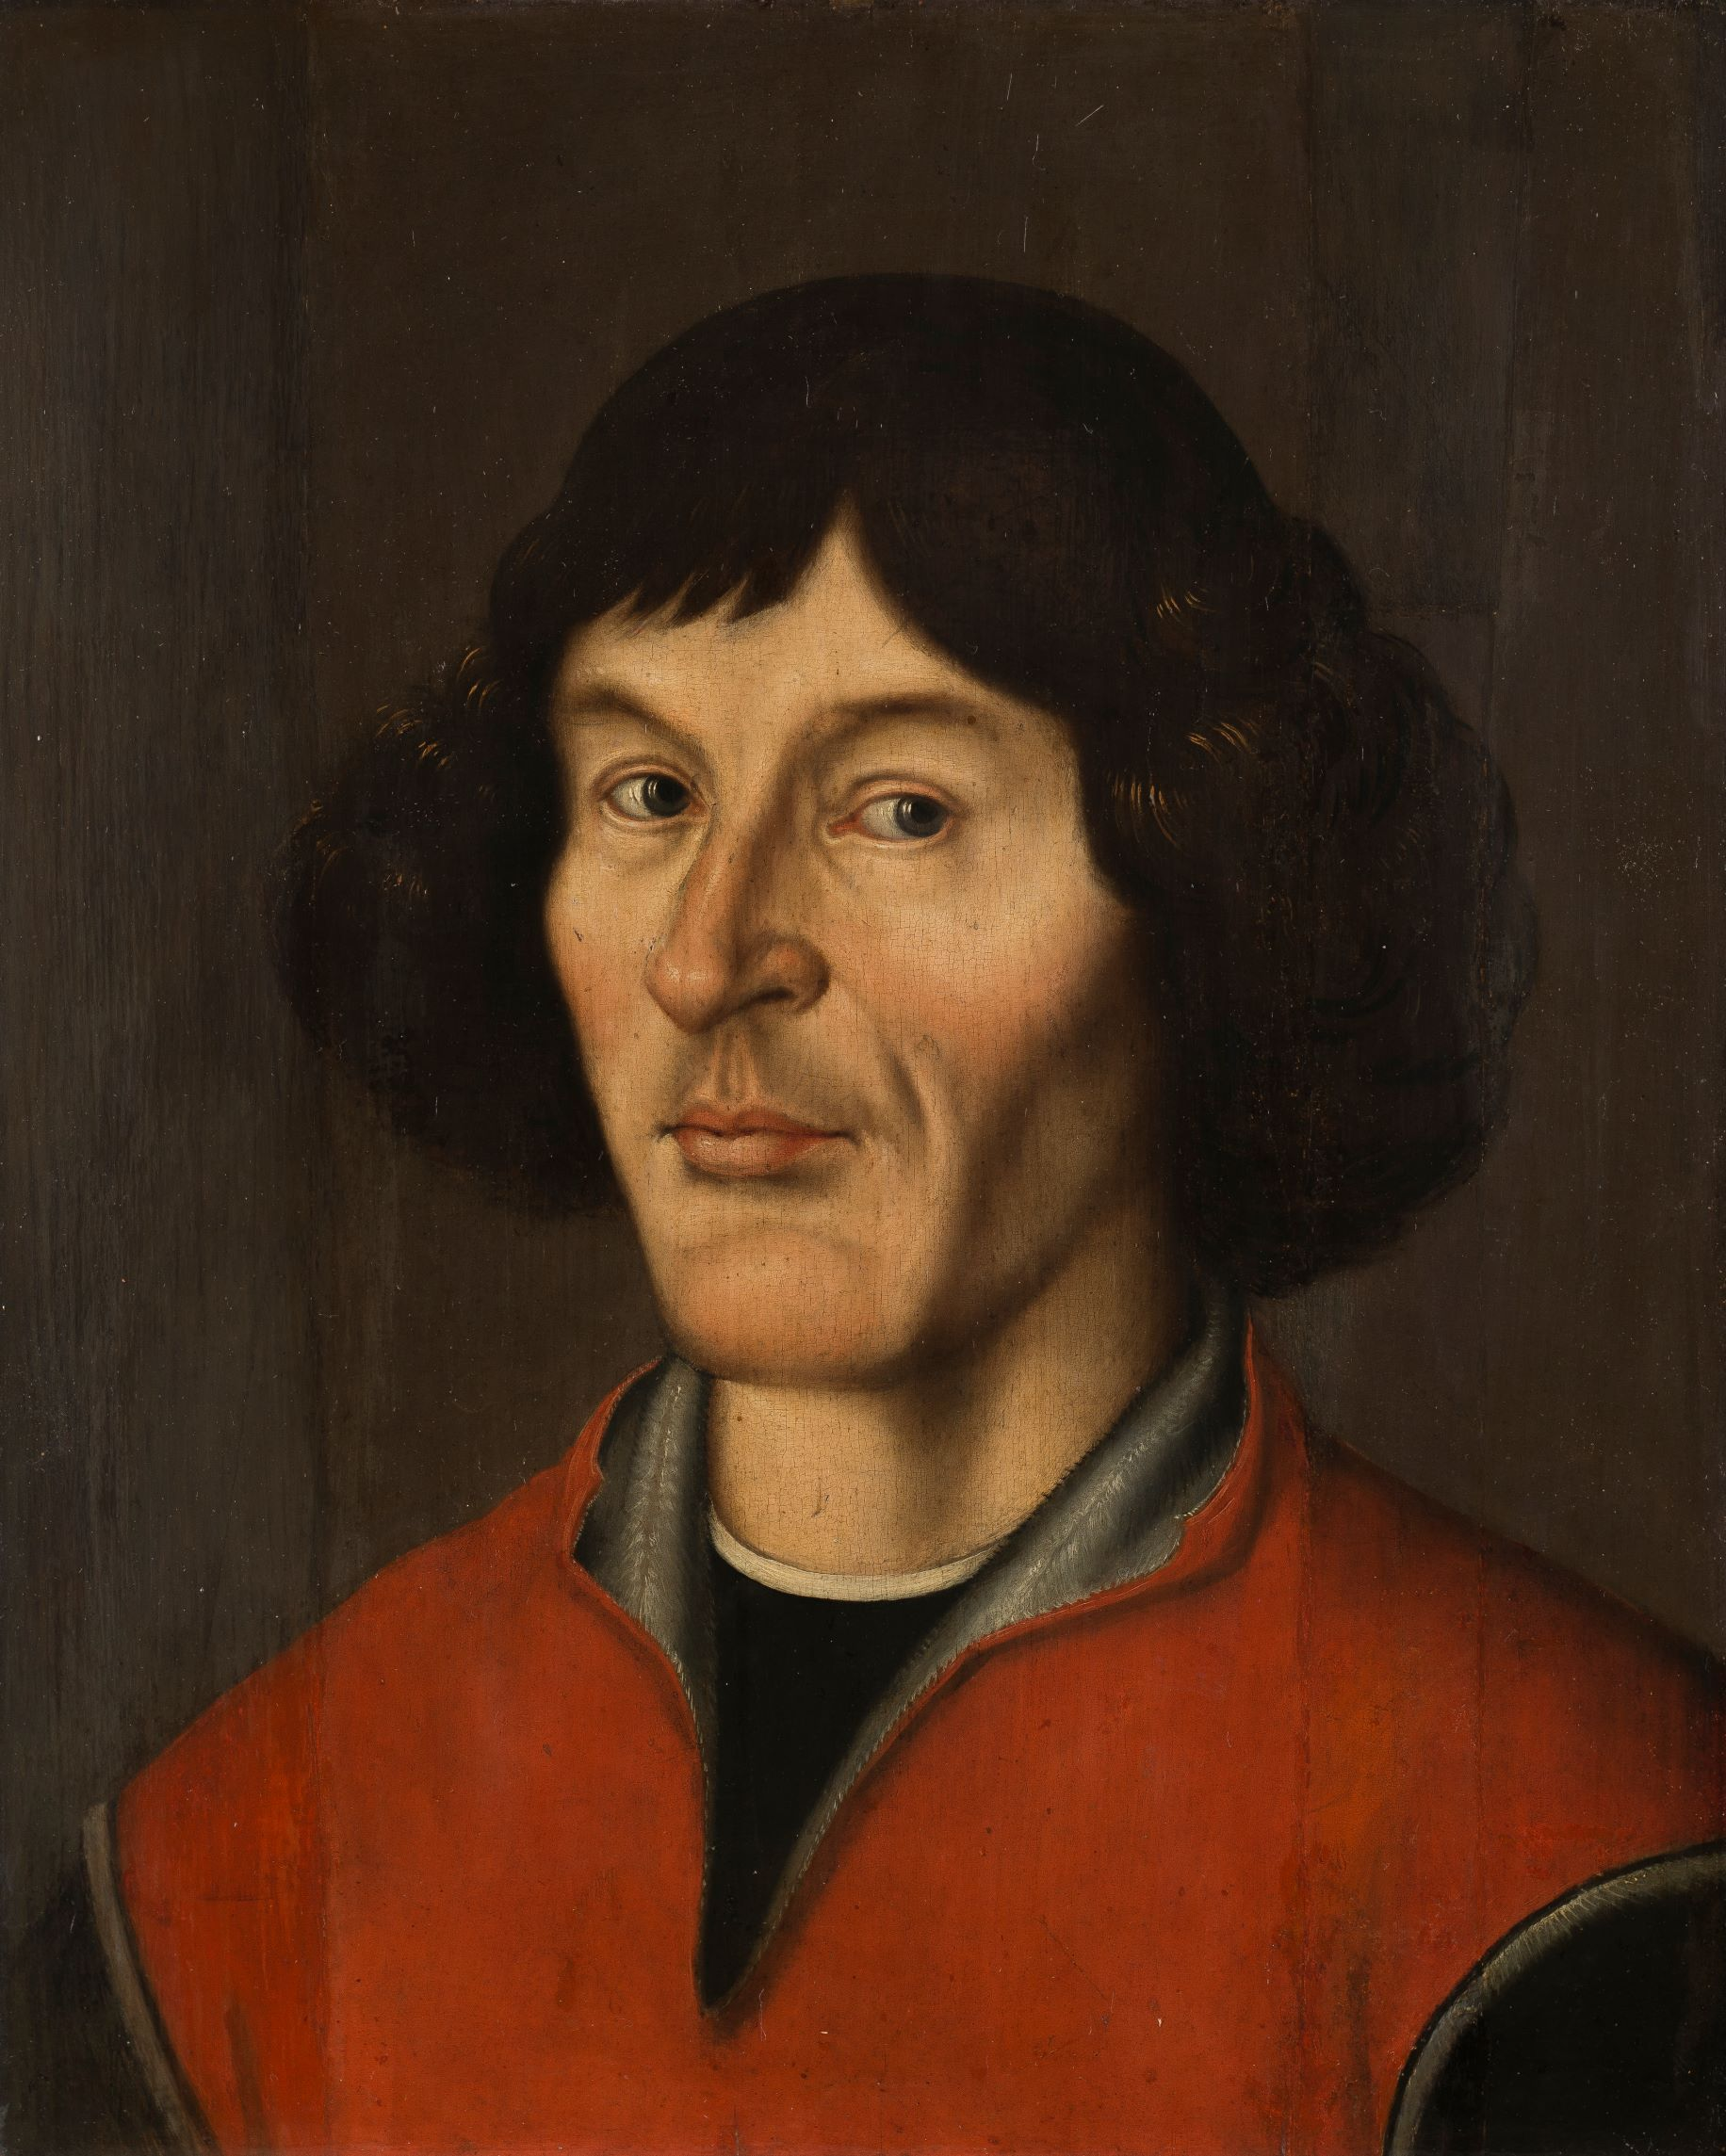
\includegraphics[width=1.0\textwidth]{pictures/copernicus.jpg}
      \captionof{figure}{Nicolaus Copernicus (\textit{Britannica})}
    \end{center}
  \end{columns}
\end{frame}

\begin{frame}
  \frametitle{Copernicus' Heliocentric System}
  \begin{columns}
    \column{0.40\textwidth}
    Based on the Ptolemy's geocentric system:
    \begin{itemize}
      \item Sun replaces Earth as the \textcolor{red}{center}.
      \item Planets arranged by \textcolor{red}{distance from the Sun}.
      \item \textcolor{red}{Retrograde motion} explained by Earth's motion, no epicycles needed.
      \item Small \textcolor{red}{epicycles} still used to refine circular orbits.
      \item He believed the Universe is still spherical and finite
    \end{itemize}

    \column{0.55\textwidth}
    \begin{alertblock}{Website}
      Visit: \textcolor{blue}{https://osp.berry.edu/CopernicanSystem.html}
    \end{alertblock}
    \begin{block}{Fact}
      Initially, the heliocentric model was only a \textcolor{red}{mathematical hypothesis}.
    \end{block}
  \end{columns}
\end{frame}

\begin{frame}
  \frametitle{Tycho Brahe}
  \begin{columns}
    \column{0.50\textwidth}
    \begin{itemize}
      \item Built \textcolor{red}{advanced observatories}.
      \item Collected the most \textcolor{red}{precise astronomical data}.
      \item Proposed a \textcolor{red}{hybrid model}:
      \begin{itemize}
        \item Sun orbits Earth
        \item Other planets orbit Sun
      \end{itemize}
      \item Data later allowed \textcolor{red}{Kepler} to formulate his laws.
    \end{itemize}
    \begin{block}{Google}
      Go to the Third link in my tab!
      
    \end{block}
    \column{0.45\textwidth}
    \begin{center}
      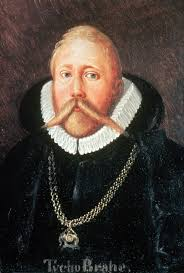
\includegraphics[width=0.6\textwidth]{pictures/tycho.jpg}
      \captionof{figure}{Tycho Brahe (\textit{Britannica})}
    \end{center}
  \end{columns}
  \begin{alertblock}{Interesting fact}
    He died from a ruptured bladder after holding in his urine.
  \end{alertblock}
\end{frame}

\begin{frame}
  \frametitle{Johannes Kepler}
  \begin{columns}
    \column{0.50\textwidth}
    \begin{itemize}
      \item Student of \textcolor{red}{Tycho Brahe}.
      \item Used precise data to show \textcolor{red}{planetary orbits are elliptical}.
      \item \textcolor{red}{Kepler's Three Laws of Planetary Motion}:
      \begin{itemize}
        \item Elliptical orbits with Sun at one focus.
        \item Equal areas in equal times.
        \item Square of orbital period $\propto$ cube of distance from Sun.
      \end{itemize}
      \item Provided mathematical proof for \textcolor{red}{heliocentrism}.
    \end{itemize}
    \begin{block}{Google}
      Go to the Fourth link in my tab!
    \end{block}

    \column{0.45\textwidth}
    \begin{center}
      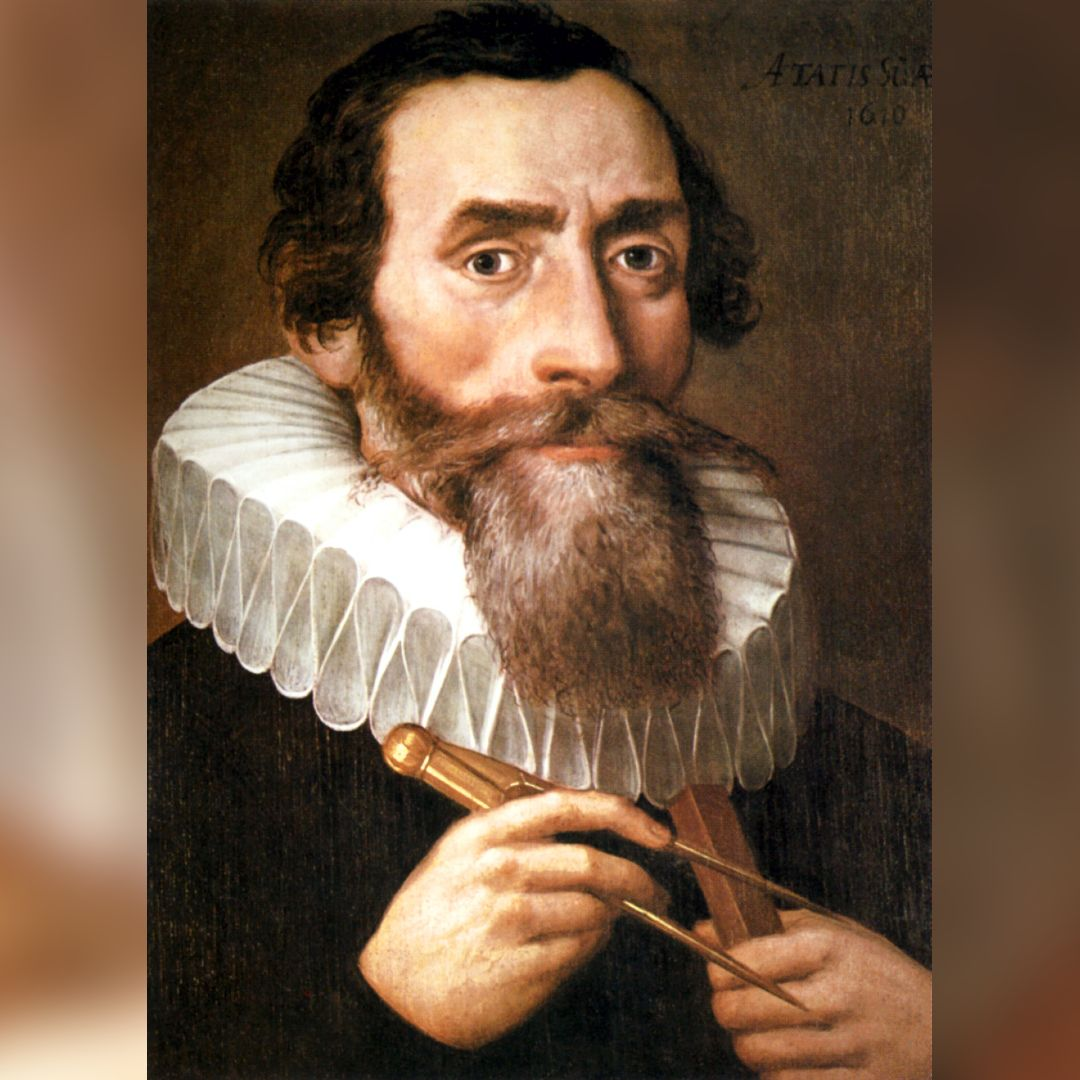
\includegraphics[width=0.9\textwidth]{pictures/kepler.jpg}
      \captionof{figure}{Johannes Kepler (\textit{space})}
    \end{center}
  \end{columns}
  \begin{alertblock}{Interesting fact}
    He was owed wages for 20 years and died on the way to get his wages.
  \end{alertblock}
\end{frame}

\begin{frame}
  \frametitle{Galileo Galilei}
  \begin{columns}
    \column{0.55\textwidth}
    \begin{itemize}
      \item First to use a \textcolor{red}{telescope} to observe the universe.
      \item Discovered four moons orbiting \textcolor{red}{Jupiter}.
      \item Publicly challenged \textcolor{red}{geocentric model}.
      \item Faced opposition from the \textcolor{red}{Catholic Church} for contradicting the Bible.
      \item He suggested that our universe is not a dome
    \end{itemize}

    \begin{block}{Interesting Fact}
      The Bible teaches how to go to heaven, not how the heavens go.
    \end{block}

    \column{0.40\textwidth}
    \begin{center}
      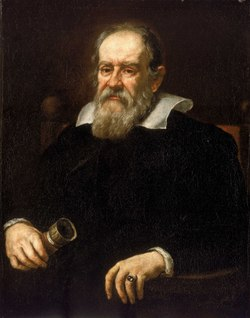
\includegraphics[width=0.9\textwidth]{pictures/galilei.jpg}
      \captionof{figure}{Galileo Galilei (\textit{Britannica})}
    \end{center}
  \end{columns}
\end{frame}

\begin{frame}
  \frametitle{Dialogue Concerning the Two Chief World Systems}
  \begin{columns}
    \column{0.55\textwidth}
    \begin{itemize}
      \item Pope Urban VIII supported Galileo to introduce both systems.
      \item Book compares Ptolemaic and Copernican systems.
      \item Written as a conversation between:
      \begin{itemize}
        \item Salviati - defends heliocentrism.
        \item Simplicio - supports geocentrism.
        \item Sagredo - neutral observer.
      \end{itemize}
      \item Written in \textcolor{red}{Italian}, accessible to general public.
    \end{itemize}

    \column{0.40\textwidth}
    \begin{center}
      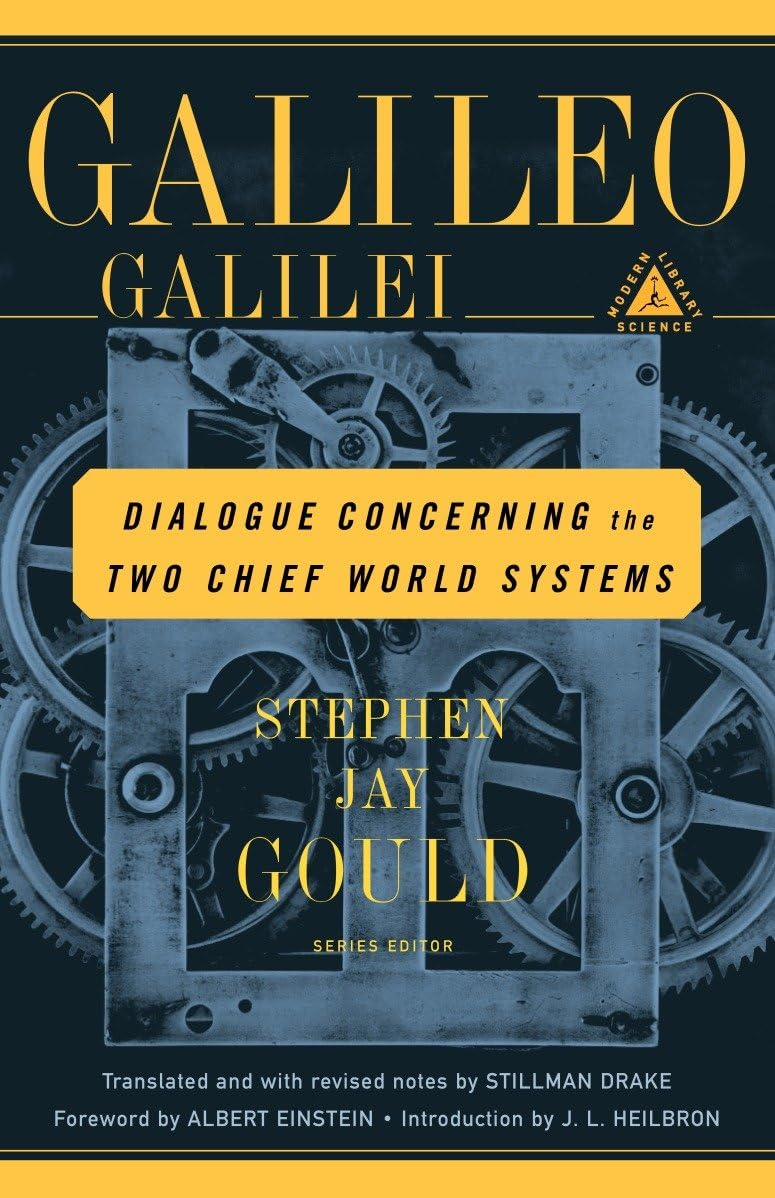
\includegraphics[width=0.8\textwidth]{pictures/dialogue.jpg}
      \captionof{figure}{Dialogue Concerning the Two Chief World Systems by Galileo}
    \end{center}
  \end{columns}
\end{frame}

\begin{frame}
  \frametitle{After the Dialogue}
  \begin{center}
    \begin{itemize}
      \item Book seen as an attack on the Pope and Catholic authority.
      \item Galileo forced to recant heliocentrism, condemned as \textcolor{red}{"vehemently suspected of heresy"}.
      \item Sentenced to \textcolor{red}{lifetime house arrest} in Florence, but continued his studies.
    \end{itemize}
  \end{center}
\end{frame}

\begin{frame}
\frametitle{Student Activity: Fill in the Scientist Names and Create a Timeline}

\textbf{Instructions:}  
1. Use the word bank to fill in the blank names.  
2. Once completed, arrange the scientists in \textbf{chronological order} on a timeline.

\vspace{0.3cm}

\textbf{Word Bank:} Eudoxus, Aristotle, Ptolemy, Copernicus, Tycho Brahe, Kepler, Galileo Galilei

\vspace{0.3cm}

\begin{enumerate}
    \item \_\_\_\_\_\_ developed \textbf{concentric spheres} to explain planetary motion.  
    \item \_\_\_\_\_\_ used a \textbf{telescope} to observe moons of Jupiter, phases of Venus, and publicly supported heliocentrism.  
    \item \_\_\_\_\_\_ proposed a \textbf{Sun-centered (heliocentric) universe} with circular orbits, still keeping some small epicycles.  
    \item \_\_\_\_\_\_ wrote the \textbf{Almagest} and introduced \textbf{epicycles} to explain \textbf{retrograde motion}.  
    \item \_\_\_\_\_\_ formulated \textbf{Kepler's laws of planetary motion}: elliptical orbits, equal areas in equal times, period-distance law.  
    \item \_\_\_\_\_\_ built precise observatories and collected extremely accurate astronomical data.  
    \item \_\_\_\_\_\_ proposed a \textbf{geocentric model} with a \textbf{spherical Earth} and \textbf{perfect circular orbits}.  
\end{enumerate}

\vspace{0.3cm}
\textit{Optional: Draw a simple timeline and place each scientist in chronological order.}

\end{frame}

\begin{frame}
\frametitle{Answer Key: Timeline of Astronomical Discoveries}

\textbf{Chronological Order of Scientists and Their Contributions:}

\begin{enumerate}
    \item \textbf{Eudoxus} developed \textbf{concentric spheres} to explain planetary motion.  
    \item \textbf{Aristotle} proposed a \textbf{geocentric model} with a \textbf{spherical Earth} and \textbf{perfect circular orbits}.  
    \item \textbf{Ptolemy} wrote the \textbf{Almagest} and introduced \textbf{epicycles} to explain \textbf{retrograde motion}.  
    \item \textbf{Copernicus} proposed a \textbf{Sun-centered (heliocentric) universe} with circular orbits, still keeping some small epicycles.  
    \item \textbf{Tycho Brahe} built precise observatories and collected extremely accurate astronomical data.  
    \item \textbf{Kepler} formulated \textbf{Kepler's laws of planetary motion}: elliptical orbits, equal areas in equal times, period-distance law.  
    \item \textbf{Galileo Galilei} used a \textbf{telescope} to observe moons of Jupiter, phases of Venus, and publicly supported heliocentrism.  
\end{enumerate}

\vspace{0.3cm}
\textit{Students can compare this with their filled-in word bank and check their timelines.}
\end{frame}

\begin{frame}
\frametitle{APA reference}
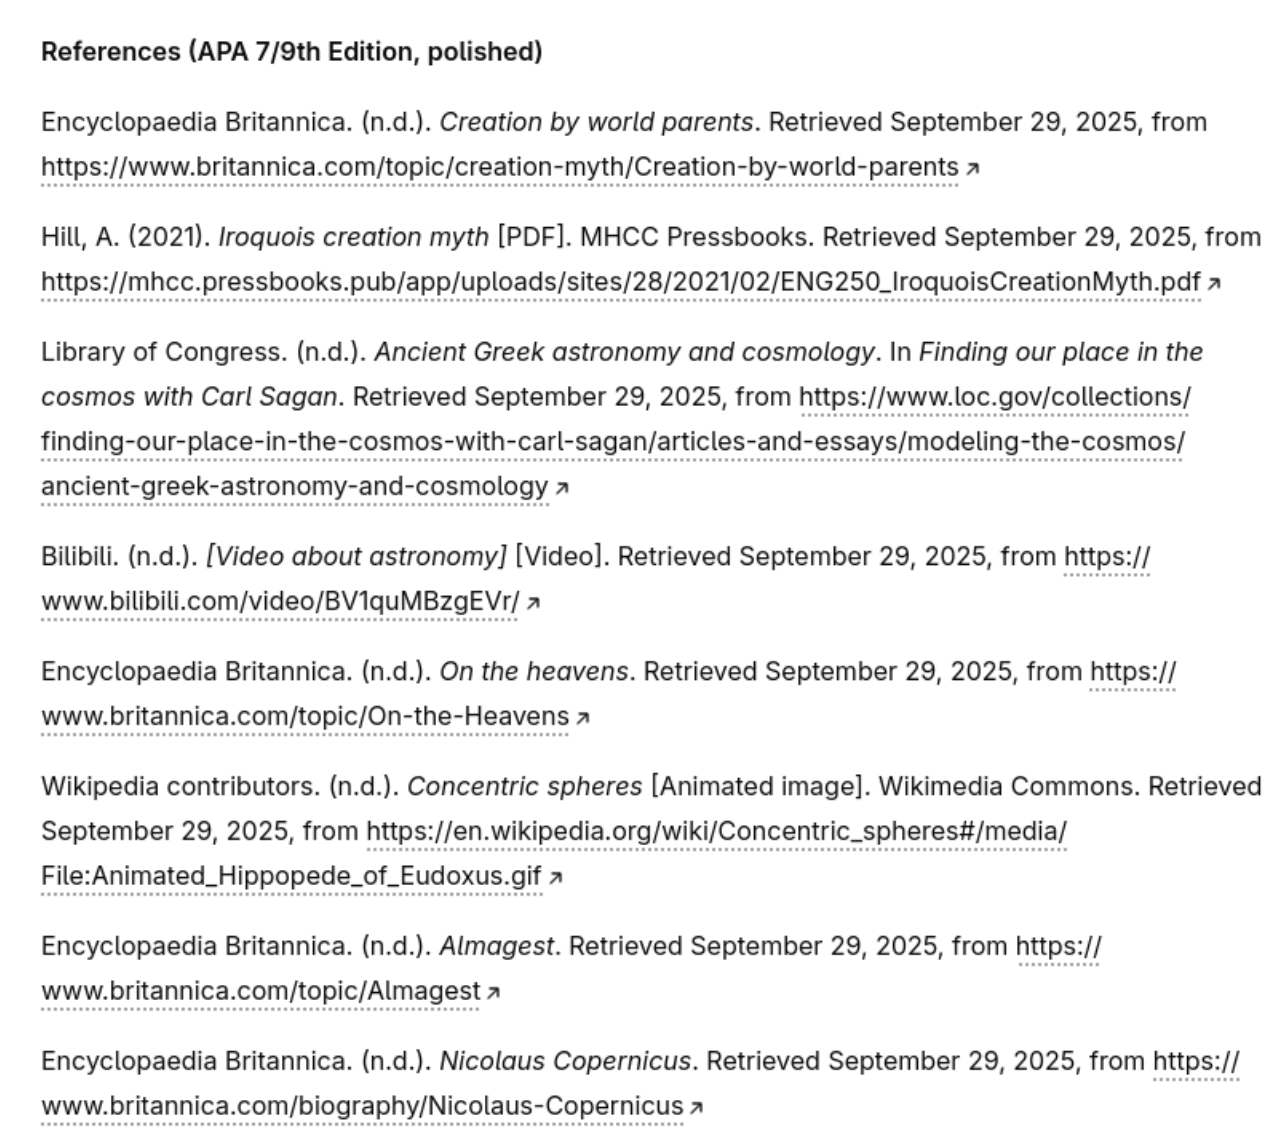
\includegraphics[width=0.612\textwidth]{pictures/2025-09-29_20-52-43.png}
\end{frame}

\begin{frame}
  \frametitle{APA reference}
  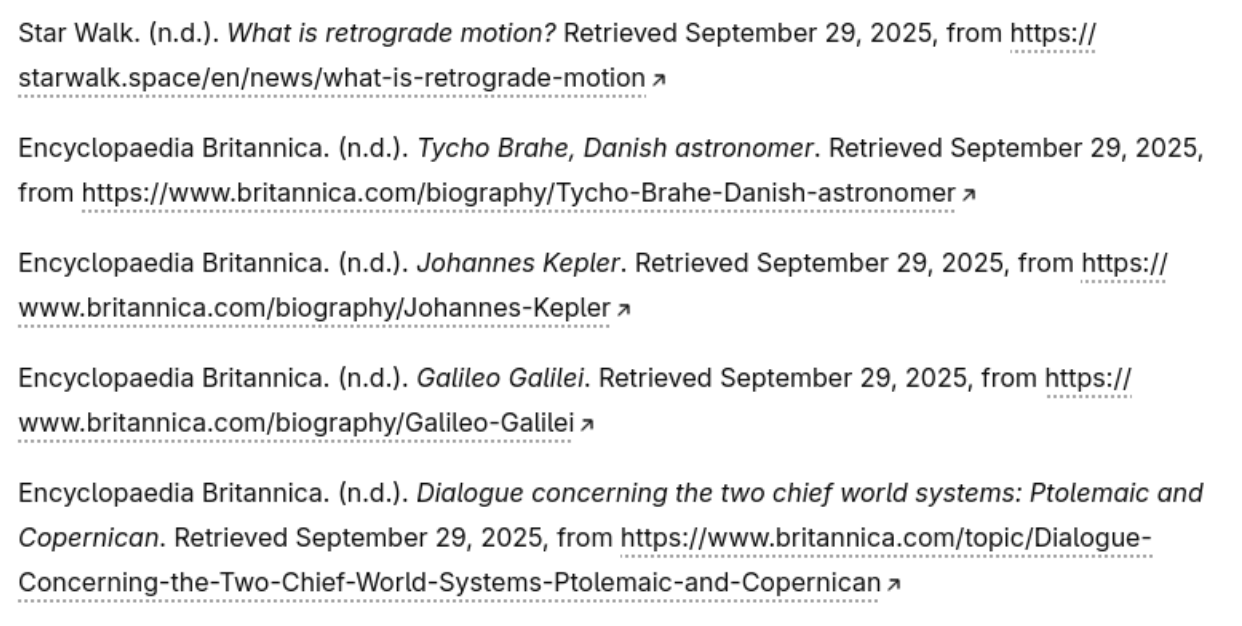
\includegraphics[width=\textwidth]{pictures/2025-09-29_20-53-39.png}
\end{frame}


\end{document}
